%\zhiyuan{Other explanations: CoT prompting is more statistically efficient, .}
 
\section{Introduction}\label{sec:intro}
 

Large Language Models (LLMs) exhibit exceptional capabilities in complex reasoning tasks such as mathematical problem-solving and code generation \citep{Chowdhery2023, anil2023palm, achiam2023gpt, FunSearch2023, trinh2024solving}, far  surpassing standard supervised machine learning techniques. The key to unlocking these advanced reasoning abilities lies in enabling LLMs to generate intermediate steps, or a chain of thought (CoT), before finalizing the final answer. This can be achieved through various methods, including training or instruction tuning a model with examples enriched with intermediate steps \citep{ling2017program, cobbe2021training, nye2021show, chung2022scaling}, or through few-shot CoT prompting \citep{reynolds2021prompt, nye2021show, wei2022chain}.

A natural explanation is that the intermediate steps provide extra information %to the LLMs
about the tasks and efficient approaches to solving, so 
that a model can imitate. %those steps and solve the tasks more effectively. 
However, intriguingly, the efficacy of generating thought steps extends to zero-shot CoT prompting~\citep{kojima2022large}, where LLMs are only instructed with the prompt ``let's think step by step'', and to even using incorrect reasoning steps in the few-shot examples~\citep{wang2022towards, madaan2022text}. %\hnote{Some other evidence about expressivity: instruction tuning with cot is better than standard instruction tuning \citep{lu2022learn}(similar to our experiments base vs cot (but they don't have hint))}%; cot enables smaller models to have similar reasoning capabilities as larger models \citep{menick2022teaching}}
%These observations indicate that the effectiveness of the original CoT prompting should not be solely attributed to its content, specifically, the semantic information encapsulated within the few-shot exemplars. Its form, which guides the LLMs to generate intermediate steps, also plays a significant role.
%\tnote{another version which I think is fine?; old version is above}
%These observations suggest that 
%in the original few-shot CoT settings, 
%the form of few-shot CoT is as important as (if not more important than) the contents in them, because merely instructing the LLMs to generate the intermediate steps helps. 
These observations suggest that
the form of CoT prompting is as important as (if not more important than) its content, because merely instructing LLMs to generate the intermediate steps helps. 

This paper aims to study why the form of CoT improves the reasoning capability of LLMs. Our hypothesis is that CoT allows for performing more serial computations that a vanilla transformer cannot do without CoT. We formulate and analyze this hypothesis through the lens of expressiveness with and without CoT. We adopt the language of circuit complexity to discuss the capability of transformers. Previous works~\citep{liu2022towards,merrill2023parallelism} have shown standard decoder-only transformers (that output answers directly) are efficient parallel computers and can only express functions computable in an $O(1)$-parallel run-time with threshold circuits, $\TC^0$, a computational model that allows the $\AND$, $\OR$, $\NOT$ and $\MAJORITY$ function with multiple inputs to be computed efficiently in parallel. 
We first show a tighter upper bound (\Cref{thm:AC0_upper_bound}) for expressiveness of constant-precision transformer -- it can only express a proper subset class of $\TC^0$, $\AC^0$, where $\MAJORITY$ gates are not allowed. Our upper bound is also more realistic because it handles the rounding issue or iterative addition of floating point numbers, while most previous results essentially only work for fixed-point number addition.


We then show that transformers equipped with CoT---allowing the transformer to auto-regressively generate a sequence of intermediate tokens before answering the questions---can solve complex problems that inherently require serial computations (assuming well-known conjectures in complexity theory). Intuitively, without CoT, the number of serial computations conducted by the transformer is bounded by the depth (which is considered as a fixed constant for this work), whereas with $T$ intermediate steps, the number of serial computations possible is boosted to $T$. Note that $T$ can easily increase as the sequence length increases where the depth is a fixed number that depends on the architecture. 
%\zhiyuan{@tengyu: the last sentence is incorrect technically. Maybe delete. The major difference is the one step of parallel computation within a forward pass can have as many intermediate outputs as the embedding size, but CoT only allows you to output one bit/token.} \tnote{are we talking about the same thing? "Note that $k$ can easily increase as the sequence length increases where $r$ is a fixed number that depends on the architecture." sounds just by definition true because $r$ is considered as fixed (e.g., GPT-4 always have r layers no matter how long the sequence is), and k is a variable} \tnote{maybe even remove ``as the sequence length increases'', which doesn't sound necessary}

Concretely, we prove that a constant-precision transformer with $T$ intermediate steps and embedding dimension logarithmic in the sequence length can express any functions computable by a circuit of size $T$ in \Cref{thm:cot_dlogn_main}. Taking $T$ to be polynomial in the sequence length, the result suggests that transformers with polynomially many intermediate steps are capable of computing all circuits in with polynomial size, $\Ppoly$, a superclass of P. \Cref{thm:cot_dlogn_main} also implies that transformers with linearly many intermediate steps can compute all regular languages, including composition of non-solvable groups, like permutation group over five elements, $S_5$, which does not belong to $\AC^0$ and is also widely conjectured to be out of $\TC^0$. As such, polynomially many CoT steps makes transformers with bounded depth and precision strictly more powerful. We define the problem class that transformers can solve with a certain amount of CoT steps formally in \Cref{defi:complexity_cot} and summarize our theoretical results in \Cref{fig:cot_diagram_constant}. Interestingly, we also show that logarithmically many CoT steps do not allow the transformer to compute functions beyond $\AC^0$. (\Cref{thm:AC0_upper_bound})

\begin{figure}[t]
\begin{center}
\vspace{-1.5cm}
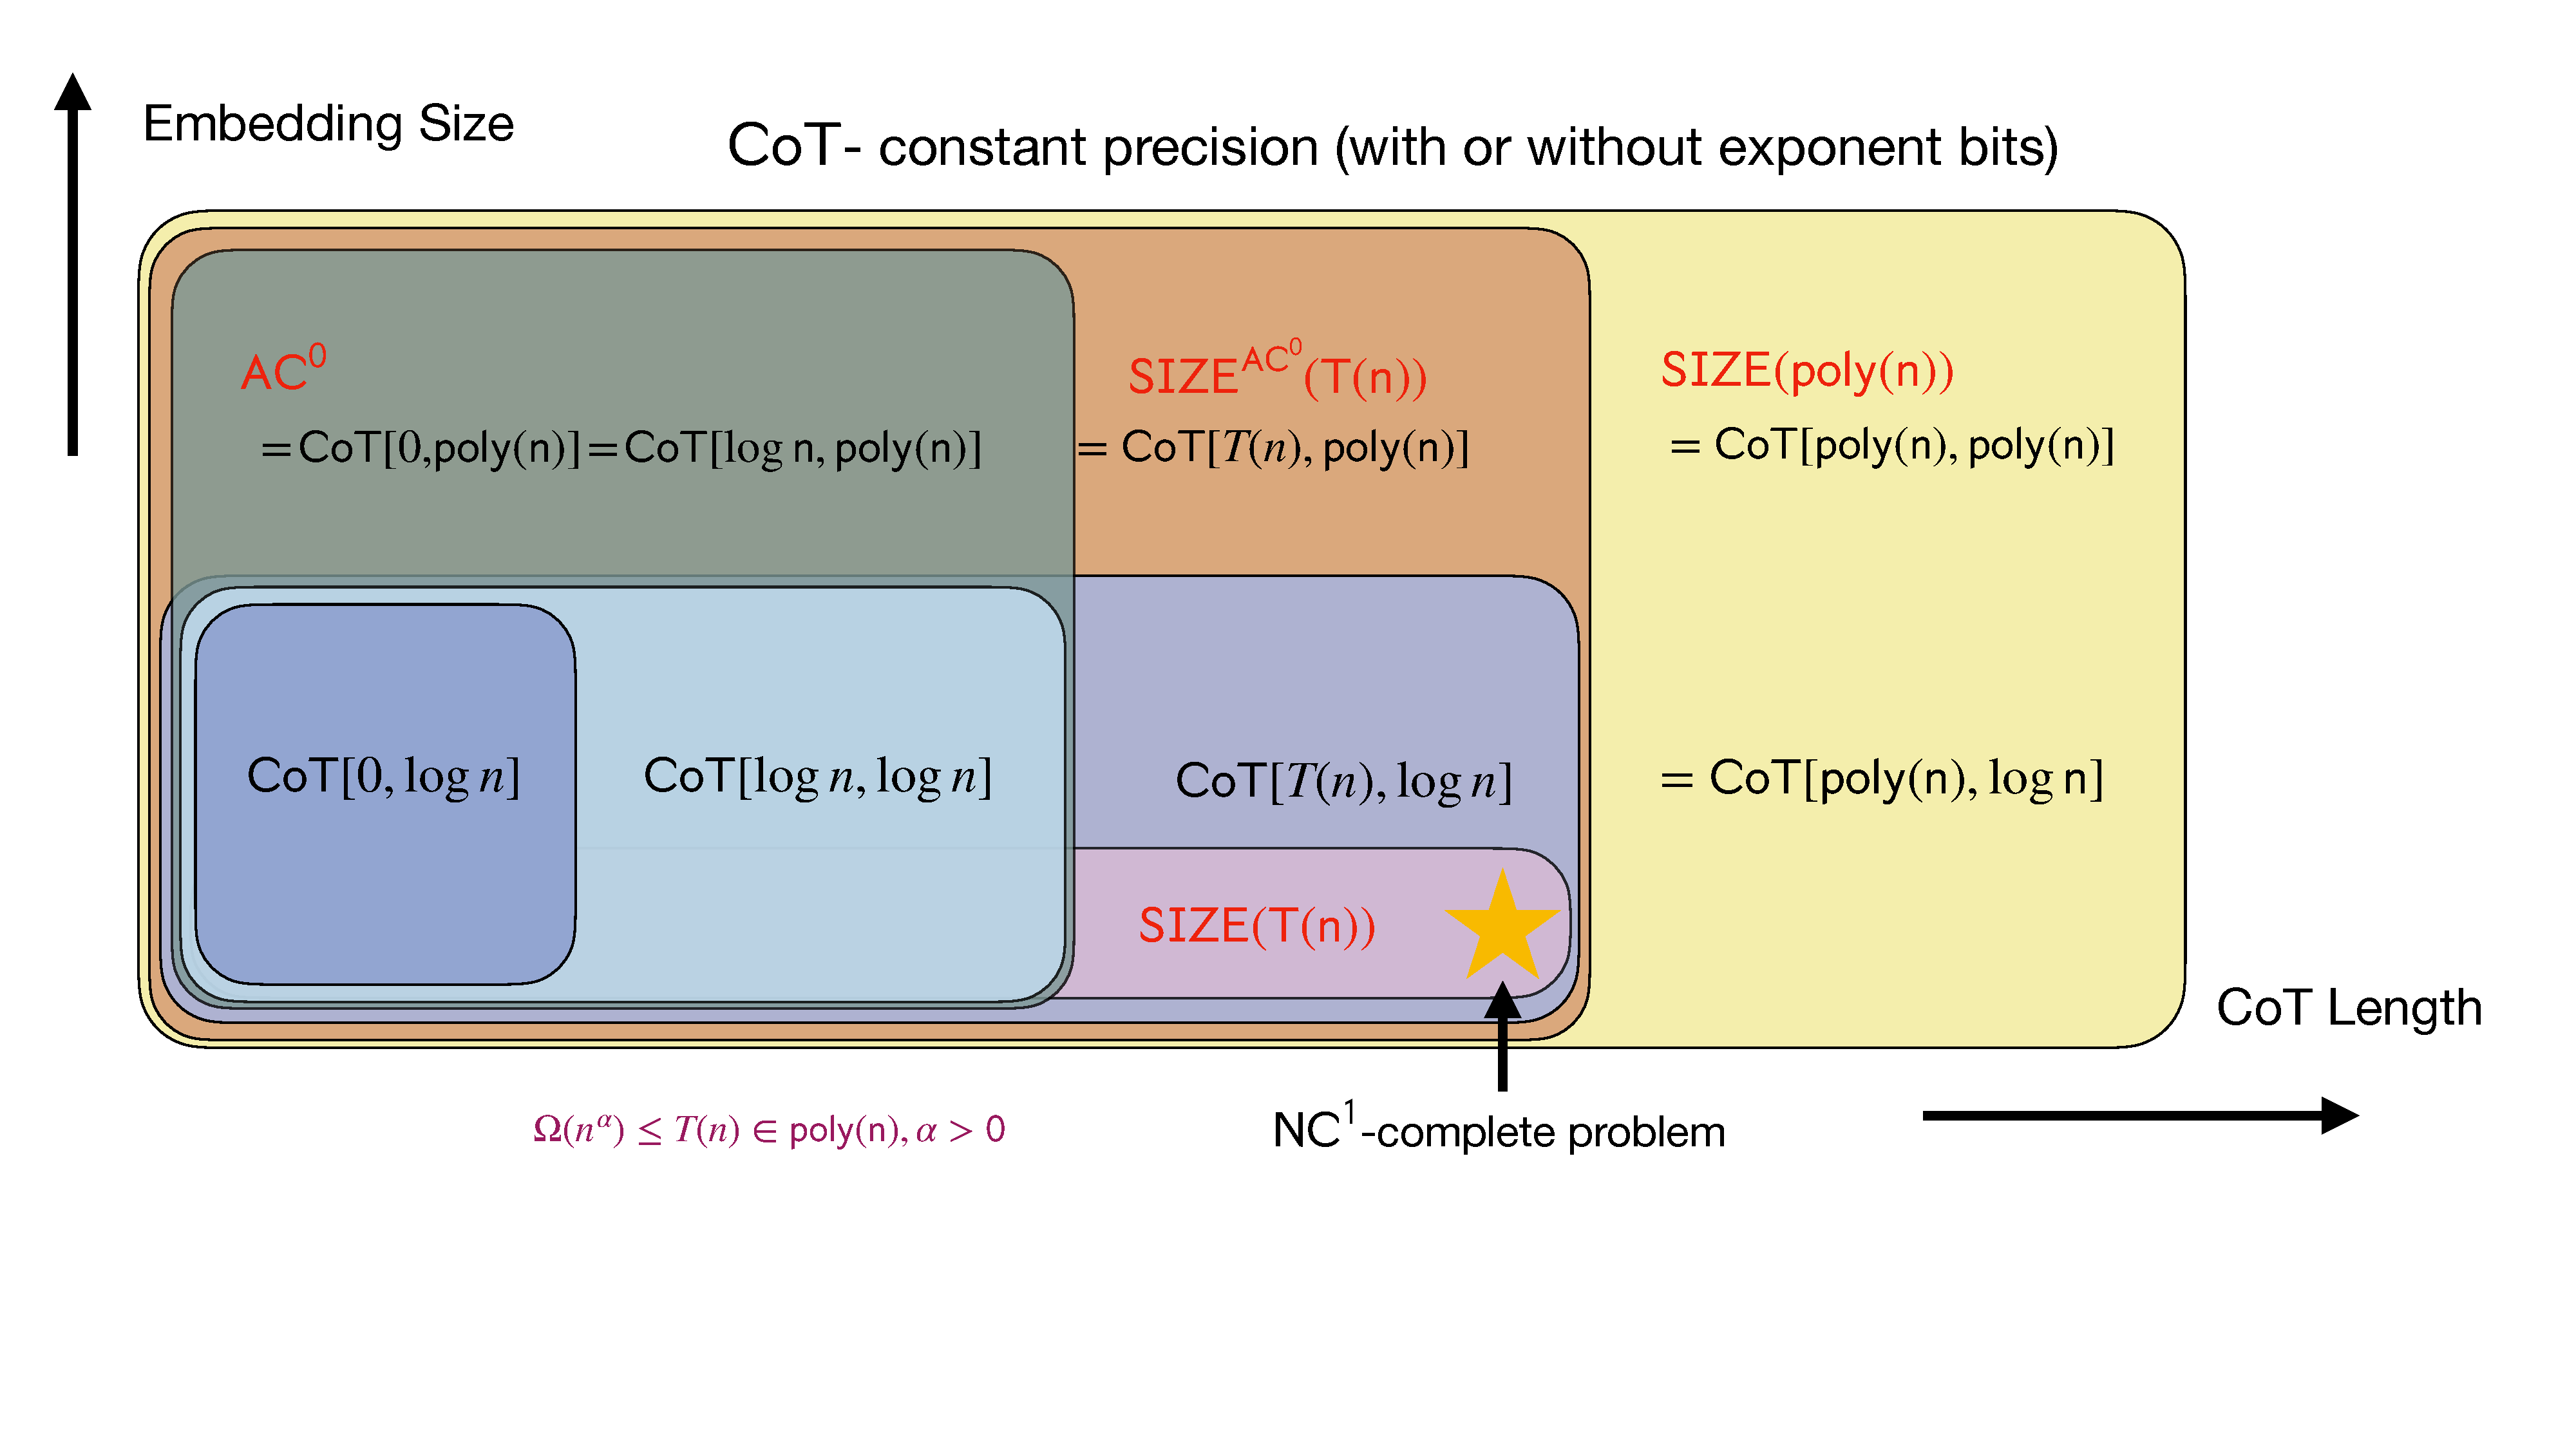
\includegraphics[width=1.1\textwidth]{figures/cot_diagram_constant.pdf}
\vspace{-2cm}
\caption{Relationship diagram between \cot complexity class with different embedding sizes $d(n)$ and CoT lengths $T(n)$. We fix the precision to be constant (the above diagram holds with or without constantly many exponent bits) and omit them in the notation for simplicity. The diagram for log precision is similar (with $\AC^0$ replaced by $\TC^0$), and is thus deferred to the appendix,~\Cref{fig:cot_diagram_log}. }\label{fig:cot_diagram_constant}
\end{center}
\end{figure}
%In contrast, \Cref{thm:AC0_upper_bound} show that transformers with CoT can only compute constant-depth polynomial-size circuits $\AC^0$, which is a strict subset of $\Ppoly$. If we allow the numerical precision of the transformer to increase logarithmically in the sequence length, \Cref{thm:TC0_upper_bound} shows that transformers with CoT can compute constant-depth circuits with threshold or majority gates, $\TC^0$, which is widely conjectured to be a strict subset of $\Ppoly$.
%Under the standard complexity theory assumption that $\TC^0$ is strictly smaller than $\Ppoly$, there exists a problem that requires inherently serial computations that can be solved by CoT but not a vanilla transformer. 

%In particular, under the stronger complexity theory assumption $\TC^0 \subsetneq  \NC^1$~\citep{yao1989circuits}, we prove that the problem of composing a sequence of permutations over $n$ items be solved by CoT with $O(n)$ intermediate steps not by vanilla constant-depth  transformers. Composing a sequence of permutations is an important special case of matrix multiplication  to  and is a prototypical question that is believed to require inherently serial computations. 

To corroborate our theoretical analysis, we empirically evaluate the capability of transformers in solving four core problems: modular addition, permutation composition, iterated squaring, and circuit value problem. 
We learn transformers to solve these tasks with a large amount of synthetic data, with and without CoT, or with additional hint but not CoT.  The modular addition belongs to $\TC^0$, meaning it can be easily solved in parallel. \citet{liu2022transformers} shows it is solvable by constant-depth transformers with log-precision and, indeed empirically depth 1 is sufficient for the parity problem (Modulo 2 addition). The other three tasks are all conjectured to require inherently serial computations. As expected, the vanilla transformer either requires a huge depth to solve these tasks (because the depth is the upper bound on the number of serial computation by transformers), or cannot solve the tasks at all. On the other hand, CoT can solve these tasks as long as the depth exceeds a small threshold. These experiments demonstrate CoT can provide more serial computations to solve complex reasoning tasks. 


%\zhiyuan{need some help with intro. The new $\AC^0$ expressiveness upper bound predicts that constant depth transformer cannot learn parity but in experiments 1-layer transformer suffices to learn parity. The reason for this mismatch between theory and experiments might be that $T$ is not large enough. \\
%
%Some intuition that why addition is not trivial when you only have constant precision. In FP16, 256+1=256 because BF16 only have 8 bit-precision}



% %that the role of the prompt here might not be allowing in-context learning of the solution hidden in the prompt, but rather encourages LLM to generate a chain of thought, which gives LLM more time and space to do computation. 

% %If certain problems cannot be computed by LLMs directly without using extra time or space, then invoking CoT before answering the problem could improve the accuracy by avoiding those direct answers which have to be wrong. However, to our best knowledge, such intuition has never been  rigorously justified. Thus it is natural to ask the following questions:
%   % \begin{quote}
%   % 	  Is there a provable benefit of CoT in terms of the expressiveness of LLMs? If so, what problems does CoT enable LLMs to solve?
%   % \end{quote}

% \subsection{Our results}
% In this paper, we give both positive answers to the above questions. High-level speaking, we show CoT empowers the transformer the ability to solve inherently serial problems, and that the lower the transformer depth is, the larger the benefit the transformer received from using CoT. It is shown by \citet{liu2022transformers} (restated as \Cref{thm:TC0_upper_bound}) that  constant-depth transformers without CoT, even with an embedding size polynomial to the input sequence length, can only solve problems within $\TC^0$, that is, the problems solvable by constant-depth poly-size circuits with threshold gates. Thus, low-depth transformer, no matter how large the embedding size is, can not solve those inherently serial problems. 

% Our first theoretical contribution is the following theorem, which says that CoT allows transformer to solve inherently serial problems, and the expressiveness of the transformer directly relates to the number of CoT allowed.

% \begin{theorem}\label{thm:intro_Ppoly}
% For any problem solvable by boolean circuits of size $T(n)$, it is solvable by some  2-layer decoder-only transformer with finite precision, $O(\log n)$ embedding size,  and trainable position encoding using $T(n)$ steps of CoT. 
% \end{theorem}

% As an implication of the above theorem, we can prove an expressiveness separation between transformers with $O(n)$ steps of CoT and without CoT.

% \begin{theorem}\label{thm:intro_Ppoly}
%    Under some standard hardness assumption, there is some matrix multiplication problem that cannot be solved constant-depth circuit without CoT, but can be solved if $O(n)$ steps of CoT is allowed.
% \end{theorem}
% \zhiyuan{ which is equal to the following}
% \begin{theorem}\label{thm:cot_0_n_separation}
%     Under the assumption $\TC^0\subsetneq \NC^1$, it holds that $\T[\log(n)] = \Cot[0][\log(n)]\subsetneq \Cot[n][\log(n)]$.
% \end{theorem}


% Beyond transformers with $O(\log n)$ embedding size, we also give a complete characterization for the expressiveness of constant-depth transformers with $O(\poly( n))$ embedding size and any steps of CoT. 

% \begin{theorem}\label{thm:cot_dpolyn_slogn_main}
% For any function $T:\mathbb{N}^+\to \mathbb{N}^+$, $\SIZE^{\TC^0}(T(n)) = \Cot[T(n)][ \poly(n)]$.	
% \end{theorem}


%  Here $\SIZE^{\TC^0}(T(n))$ means a size $T(n)$ boolean circuit with $\TC^0$ oracles. In other words, each gate in this size $T(n)$ circuit could be as powerful as a constant-depth, poly size circuit with threshold gates, which is a very strong parallel computer. And $T(n)$ steps of CoT allows us to run $T(n)$ different constant-step polysize parallel computers sequentially!

% Besides theoretical contributions, we also empirically investigate the expressiveness of the transformers on 4 different arithmetic problems with increasing difficulty for parallel computer. Our experiments suggest that turning on CoT drastically improves the expressiveness of low-depth transformers on problems which are hard to be parallel computed, \emph{i.e.}, those inherently serial problems.    